\input{../slides/common/slides_common}

\newif\ifbook
\input{../shared/chisel}

% TikZ for diagrams
\usepackage{tikz}
\usetikzlibrary{positioning, arrows.meta}

% Optional visual tweaks
\tikzset{
    >=Stealth,
    every node/.style={rounded corners=2pt}
}

\title{Agile Hardware Design}
\author{Martin Schoeberl}
\date{\today}
\institute{Technical University of Denmark\\
Embedded Systems Engineering}

\begin{document}

\begin{frame}
\titlepage
\end{frame}


\begin{frame}[fragile]{TODO}
\begin{itemize}
\item Scala/Chisel/Module
\item Functional programming
\item Generator examples
\item Check my normal Chisel book on the topic
\item Test arbiter code
\item Find a third lab topic
\end{itemize}
\end{frame}

\begin{frame}[fragile]{Lecture 1}
\begin{itemize}
\item Waterfall and Agile design style
\item Quick overview of Chisel and Scala
\item Functional programming in Scala
\item Links to further reading and material
\end{itemize}
\end{frame}

% Week 1: Intro to Agile + Chisel

% --- Slide 1: Waterfall Model (Description) ---
\begin{frame}{The Classic Waterfall Model}
\begin{itemize}
    \item Traditional project management approach for software and hardware
    \item Development phases are sequential:
    \begin{enumerate}
        \item Requirements
        \item Design
        \item Implementation
        \item Verification
        \item Maintenance
    \end{enumerate}
    \item Each phase must be completed before moving to the next
    \item Changes are costly once early phases are complete
\end{itemize}
\end{frame}

\begin{frame}{Waterfall Model Diagram}
\centering
\resizebox{0.8\linewidth}{!}{%
\begin{tikzpicture}[
    node distance=1.4cm,
    every node/.style={draw, minimum width=3.2cm, minimum height=1.2cm, align=center}
]
\node[thick] (req) {Requirements};
\node[thick] (design) [below right=0.8cm and 0.6cm of req] {Design};
\node[thick] (impl) [below right=0.8cm and 0.6cm of design] {Implementation};
\node[thick] (verif) [below right=0.8cm and 0.6cm of impl] {Verification};
\node[thick] (maint) [below right=0.8cm and 0.6cm of verif] {Maintenance};

% Arrows
\draw[->, thick] (req.south east) -- (design.north west);
\draw[->, thick] (design.south east) -- (impl.north west);
\draw[->, thick] (impl.south east) -- (verif.north west);
\draw[->, thick] (verif.south east) -- (maint.north west);

% Feedback arrows
\draw[->, dashed, red] (design.west) .. controls +( -2,0) and +(-2,0) .. (req.west) node[midway,left]{Costly change};
\draw[->, dashed, red] (impl.west) .. controls +( -2,0) and +(-2,0) .. (design.west);
\draw[->, dashed, red] (verif.west) .. controls +( -2,0) and +(-2,0) .. (impl.west);

\end{tikzpicture}%
}
\end{frame}

% --- Slide 3: Waterfall Limitations ---
\begin{frame}{Limitations of the Waterfall Model}
\begin{itemize}
    \item Assumes requirements are fixed at the start
    \item Poor adaptability to changing customer needs
    \item Testing and feedback happen late in the process
    \item High risk of discovering major flaws late
    \item Not well-suited for rapid prototyping or exploratory projects
\end{itemize}
\end{frame}


\begin{frame}{Why Agile for Hardware?}
\begin{itemize}
    \item Traditional hardware development: long, rigid cycles
    \item Software has embraced Agile:
    \begin{itemize}
        \item Quick iterations
        \item Test-driven development
        \item Continuous integration
    \end{itemize}
    \item Hardware complexity is increasing $\rightarrow$ need for agility!
\end{itemize}
\end{frame}

\begin{frame}{Agile Iteration Cycle}
\centering
\resizebox{0.65\linewidth}{!}{%
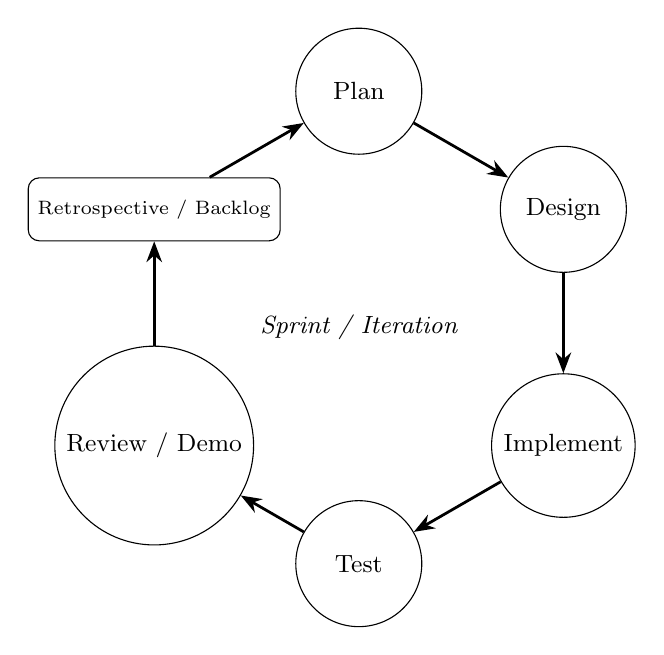
\begin{tikzpicture}[
  circular/.style={circle, draw, minimum size=1.6cm, font=\small, align=center},
  arrowstyle/.style={-Stealth, line width=1pt}
]
  % Place nodes in a circular layout
  \node[circular] (plan)      at (90:3cm)  {Plan};
  \node[circular] (design)    at (30:3cm)  {Design};
  \node[circular] (implement) at (-30:3cm) {Implement};
  \node[circular] (test)      at (-90:3cm) {Test};
  \node[circular] (review)    at (-150:3cm) {Review / Demo};
  \node[rectangle, draw, rounded corners, minimum width=3.2cm, minimum height=0.8cm, font=\scriptsize] (retro) at (-210:3cm) {Retrospective / Backlog};

  % Loop arrows
  \draw[arrowstyle] (plan) -- (design);
  \draw[arrowstyle] (design) -- (implement);
  \draw[arrowstyle] (implement) -- (test);
  \draw[arrowstyle] (test) -- (review);
  \draw[arrowstyle] (review) -- (retro);
  \draw[arrowstyle] (retro) -- (plan);

  % Central label
  \node at (0,0) [font=\small\itshape] {Sprint / Iteration};
\end{tikzpicture}%
}
\end{frame}
% --- Slide 1 ---
\begin{frame}{Agile Iteration Phases (1/3)}
\textbf{Plan}
\begin{itemize}
    \item Define goals for the upcoming sprint (typically 1-4 weeks)
    \item Select features or fixes from the product backlog
    \item Break down tasks into manageable user stories
    \item Ensure each story has clear acceptance criteria
\end{itemize}

\medskip
\textbf{Design}
\begin{itemize}
    \item Create a simple, implementable hardware design
    \item Define interfaces and parameters
    \item Update documentation and diagrams
    \item Keep the design minimal to support fast iteration
    \item Think: minimal viable product
\end{itemize}
\end{frame}

% --- Slide 2 ---
\begin{frame}{Agile Iteration Phases (2/3)}
\textbf{Implement}
\begin{itemize}
    \item Write Chisel modules for new or updated functionality
    \item Commit early and often to version control
    \item Follow coding standards and naming conventions
    \item Collaborate closely to avoid merge conflicts
\end{itemize}

\medskip
\textbf{Test}
\begin{itemize}
    \item Use automated tests (e.g., \texttt{chiseltest}) to validate functionality
    \item Run both unit tests and integration tests
    \item Include corner cases and property-based checks
    \item Maintain high test coverage throughout development
\end{itemize}
\end{frame}

% --- Slide 3 ---
\begin{frame}{Agile Iteration Phases (3/3)}
\textbf{Review / Demo}
\begin{itemize}
    \item Present completed work to the team or stakeholders
    \item Demonstrate working features in simulation or on FPGA
    \item Gather feedback on design choices and implementation
\end{itemize}

\medskip
\textbf{Retrospective / Backlog Refinement}
\begin{itemize}
    \item Reflect on what worked well and what can be improved
    \item Adjust processes, tools, and team coordination as needed
    \item Update the product backlog with new ideas or changes
    \item Prepare for the next sprint cycle
\end{itemize}
\end{frame}

\begin{frame}{Hardware Design Today}
\begin{itemize}
    \item VHDL / Verilog = rigid, low-level
    \item Hard to reuse and test modularly
    \item Long simulation cycles
    \item Not optimized for iteration or testing early
\end{itemize}
\end{frame}

\begin{frame}{Software-Inspired Hardware Flow}
\begin{enumerate}
    \item Write modular, parameterized designs
    \item Test-first using simulation
    \item Version control and CI
    \item Frequent review and refactor
    \item Code reviews and pull requests
\end{enumerate}
\end{frame}

\begin{frame}[fragile]{Chisel}
\begin{itemize}
\item A hardware \emph{construction} language
\begin{itemize}
\item Constructing Hardware in a Scala Embedded Language
\item If it compiles, it is synthesizable hardware 
\item Say goodbye to your unintended latches
\end{itemize}
\item Chisel is not a high-level synthesis language
\item Single source for two targets
\begin{itemize}
\item Cycle accurate simulation (testing)
\item Verilog for synthesis
\end{itemize}
\item Embedded in Scala
\begin{itemize}
\item Full power of Scala available
\item We use Scala to write the generators
\end{itemize}
\item Developed at UC Berkeley
\end{itemize}
\end{frame}

\begin{frame}[fragile]{The C Language Family}

\Tree[.C [
   [.{\bf Verilog} {\bf SystemVerilog} ]
   [.C++  \emph{SystemC}  ]
   [.Java [.Scala {\bf Chisel} ] ]
   [.C\# ] ] ]
 
\end{frame}

%\begin{frame}[fragile]{What Language do You Already Know?}
%\begin{itemize}
%\item ???
%\end{itemize}
%\end{frame}


\begin{frame}[fragile]{A Small Language}
\begin{itemize}
\item Chisel is a \emph{small} language
\item On purpose
\item Not many constructs to remember
\item The \href{https://github.com/freechipsproject/chisel-cheatsheet/releases/latest/download/chisel_cheatsheet.pdf}{Chisel Cheatsheet} fits on two pages
\item The power comes with Scala for circuit generators
\item With Scala, Chisel can grow with you
\end{itemize}
\end{frame}

\begin{frame}{Chisel Advantages}
\begin{itemize}
    \item Parameterization: \texttt{Vec}, \texttt{Bundle}, \texttt{Module}
    \item Reuse: higher-order functions, traits
    \item Testing: tight Scala integration
    \item Ecosystem: \texttt{chiseltest}, \texttt{firrtl}, \texttt{treadle}, \texttt{verilator}
\end{itemize}
\end{frame}


\begin{frame}[fragile]{Example: 2-bit Counter}
\begin{verbatim}
class Counter extends Module {
  val io = IO(new Bundle {
    val out = Output(UInt(2.W))
  })
  val count = RegInit(0.U(2.W))
  count := count + 1.U
  io.out := count
}
\end{verbatim}
\end{frame}

\begin{frame}[fragile]{Example Test}
\begin{verbatim}
test(new Counter) { c =>
  c.io.out.expect(0.U)
  c.clock.step()
  c.io.out.expect(1.U)
  c.clock.step()
  c.io.out.expect(2.U)
}
\end{verbatim}
\end{frame}



\begin{frame}[fragile]{Tool Flow for Chisel Defined Hardware}
\begin{figure}
    \centering
    \includegraphics[scale=0.35]{../figures/flow}
\end{figure}
\end{frame}

\begin{frame}[fragile]{Chisel is a Hardware Construction Language}
\begin{itemize}
\item The code looks much like Java code
\item But it is \emph{not} a program in the usual sense
\item It represents a circuit
\item The ``program'' constructs the circuit
\item All statements are ``executed'' in parallel
\item Statement order has \emph{mostly} no meaning
\end{itemize}
\end{frame}

\begin{frame}[fragile]{A Chisel Book}
\begin{figure}
    \centering
    \href{https://github.com/schoeberl/chisel-book}{\includegraphics[scale=0.4]{../cover-small}}
\end{figure}

\begin{itemize}
\item Available in open access (as PDF)
\begin{itemize}
\item Optimized for reading on a tablet (size, hyper links)
\end{itemize}
\item Amazon can do the printout
\end{itemize}
\end{frame}





\begin{frame}[fragile]{Further Reading and Web Resources}
\begin{itemize}
\item \href{https://www.sciencedirect.com/science/article/pii/S014193312500050X}{Scala defined hardware generators for Chisel}
\begin{itemize}
\item Journal article with generator examples
\end{itemize}
\item \href{http://www.imm.dtu.dk/~masca/chisel-book.html}{Chisel book website}
\begin{itemize}
\item Information on Chisel, a bit of Scala
\item Download the free PDF
\end{itemize}
\item \href{http://www2.imm.dtu.dk/courses/02139/}{Digital design course at DTU}
\begin{itemize}
\item Slides on digital design with Chisel
\end{itemize}
\item \href{https://github.com/schoeberl/chisel-lab}{Digital design lab at DTU}
\begin{itemize}
\item Lab material for the digital design course
\item Option to train a bit on Chisel
\end{itemize}
\end{itemize}
\end{frame}


\begin{frame}[fragile]{Lab 1}
\begin{itemize}
\item I assume that you installed all tools and did lab0 as homework
\item Functional programming in Scala
\item Links to further reading and material
\end{itemize}
\end{frame}

\begin{frame}[fragile]{Lecture 2}
\begin{itemize}
\item More on Chisel
\item Functional programming for generators
\end{itemize}
\end{frame}

\begin{frame}[fragile]{Lab 2}
\begin{itemize}
\item Write an arbitration circuit (with \code{treeReduce()})
\item Introduce some fairness to the arbitration circuit
\end{itemize}
\end{frame}

\begin{frame}[fragile]{Lecture 3}
\begin{itemize}
\item Hardware generators
\end{itemize}
\end{frame}

\begin{frame}[fragile]{Lab 3}
\begin{itemize}
\item Maybe the search circuit
\end{itemize}
\end{frame}

\begin{frame}[fragile]{Summary}
\begin{itemize}
\item The world is digital
\item Processors do not get much faster -- we need to design custom hardware
\item We need a modern language for hardware/systems design for efficient/fast development
\item Chisel builds on the power of object-oriented and functional Scala
\item We shall write hardware generators
\end{itemize}
\end{frame}


\end{document}

\begin{frame}[fragile]{Title}
\begin{itemize}
\item abc
\end{itemize}
\end{frame}
